\documentclass[runningheads]{llncs}

%PACKAGES
\usepackage[utf8]{inputenc}
\usepackage{listings, xcolor}
\usepackage{graphicx} 
\usepackage{lipsum}
\usepackage{float}
\usepackage{listings-rust}
\setcounter{secnumdepth}{5}
\begin{document}
\title{Comparing FreeST, Go and Rust}
\author{Jorge Martins\inst{1} \and
Diogo Lopes\inst{1}
}
\definecolor{darkblue}{rgb}{0.0, 0.0, 0.55}
\lstset{language=Java,
numbers=none,
keywordstyle = \color{blue},
commentstyle = \color{darkblue},
breaklines = true,
showstringspaces = false,
tabsize = 4,
basicstyle=\small,
} 
\institute{Departamento de Informática da Faculdade de Ciências da Universidade de Lisboa
\email{\{fc51033,fc51058\}@alunos.fc.ul.pt}}
\nocite{*}
\maketitle
\thispagestyle{empty}
\begin{abstract}
FreeST is an experimental functional programming language being developed at LASIGE that offers primitives to thread creation and channel communication, different to those in programming languages such as Go and Rust, that are currently being appraised by their performance and reliability. Despite being different, these languages can be compared by the characteristics of their common primitives and by their learning curve. Although there are several articles comparing Rust and Go, they mainly focus in performance and reliability instead of the learning curve of each language and their approach to channel communication and thread creation. FreeST on the other hand, due to the small community working on it, is yet to be compared to the others.
In order to compare the three languages we used an algorithm that focuses on thread creation, communication using channels and thread synchronization using those same channels. To implement this algorithm we learned the three languages so that we could comment on the difficulties and different aspects of each.
This comparison is useful to understand what aspects of some languages could benefit the others and also to inform about what difficulties developers may find when writing code in each of them.
\keywords{FreeST \and Rust \and Go.}
\end{abstract}
\section{Introduction}
Rust and Go are languages that are growing in popularity due to their performance and reliability, according to the TIOBE index, and FreeST\cite{freest} on the other hand is a very recent programming language that is still being developed at LASIGE, a research center in the Faculty of Sciences of the University of Lisbon. 
In order to compare these three languages, that were completely new to each of us until the start of this project, we aimed to understand the basic concepts of each one, such as the ownership and lifetimes in Rust or the session types \cite{session} in FreeST.
When starting to learn a new language we need to understand how the basics of that language work, and therefore our initial focus was to learn those basic concepts in each language. Once we had a clear view of this concepts we focused on the concurrency primitives of these programming languages since in this project we mainly aimed to show the differences between how each one of them handles concurrency and channels communication.
To see this differences in action we used a simple algorithm simulating a communication between a customer and a travel agency that would eventually spawn a service to finish a transaction. This way, we could see in action the creation of threads, since each of these entities will run in a different thread. This algorithm also allows to see how channel communication functions in each programming language because these threads use channels as a form of communication. Finally we can see how these channels can offer thread synchronization as well.
Our goal was to implement this algorithm in Rust, Go and FreeST, in order to understand the main differences and characteristics of each language and identifying the main complications we had while learning them.
\section{Background}
\subsection{The Plane Ticket Algorithm}
In order to explore the interprocess communication through channels and thread creation, we used a simple algorithm that simulates a customer trying to buy a plane ticket from an agency, that can eventually create a service to finish the transaction with the customer. The customer, the agency and the service will be executed in different threads and will communicate through rendezvous channels, meaning 
\begin{figure}[H]
\centering
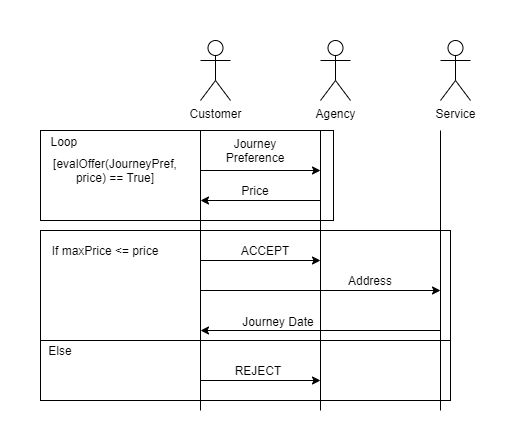
\includegraphics[scale=0.4]{Algorithm.png}
\caption{Plane Ticket Algorithm System Sequence Diagram}
\label{ssd}
\end{figure}
As we can see in figure \ref{ssd}, the algorithm consists in an early stage of negotiation where a customer will send a journey preference(e.g. "Rome") to the agency and receive the price for a ticket to the given preference repeatedly until evalOffer evaluates to true.
At this point the customer will make a choice:
\begin{itemize}
\item If the received price is lower or equal to the max accepted price of the customer, he will accept the offer.
The agency will spawn a service which will receive the customer address and send the journey date.
\item If the received price is greater than the max accepted price of the customer, he will reject the offer and end the communication.
\end{itemize}
\subsection{Programming Languages}
\subsubsection{Rust}\hfill\\\\
Rust is a programming language that greatly focuses in performance, concurrency safety and memory management.
It introduces many core features such as ownership, lifetimes and the absence of garbage collection.
Ownership is usually a new concept for programmers that is built over three simple rules:
\begin{itemize}
\item Each value in Rust has a variable that’s called its owner;
\item There can only be one owner at a time;
\item When the owner goes out of scope, the value will be dropped.
\end{itemize}
The most important rule is the 3rd. Once the lifetime of the owner of a value ends, that value is dropped in memory. This is a key aspect of the memory management model of Rust because this way we don't need to have a garbage collector like Java has, that is constantly checking if a value can be erased from memory and by doing so it has a negative impact on the performance of a program. With ownership, Rust as no need for a garbage collector and therefore its performance is greatly enhanced, being on par with languages like C and C++.\\
With ownership, once we move a variable to a function(as an argument) it stops being available to the caller:
\begin{lstlisting}[language=Rust]
fn main() {
	// s comes into scope
    let s = String::from("hello");
	// s ownership is passed to the function
    takes_ownership(s);   
    //s is not available here
}
\end{lstlisting}
Another concept that we don't usually see in other programming languages is marking a variable as mutable or immutable in its assignment. By default a variable is immutable and therefore we can change afterwards, meaning we must explicitly mark a variable as mutable in order to change it later in the program.\\
Unlike what we will see in Go and FreeST, Rust does not have primitives to create threads or channels. Therefore to do so we need to import crates that support thread creation and channels creation.\\
One of the most powerful primitives Rust has to offer are Enums, that allows a programmer to define a type by enumerating its possible variants.
\subsubsection{Go}\hfill\\\\
Go is a programming language designed at Google that focuses in performance, usability and parallel programming.
Its statically typed, meaning it checks the type safety of the program by analysing the source code. Therefore we know at compilation time what errors we might have committed.\\
It introduces a new primitive called Goroutines, a form of lightweight threads, meaning they share context with other goroutines in a program. They are also managed by the Go runtime, that will be responsible for the scheduling of each goroutine. This means that if one goroutine is blocked, Go's run-time will switch to another with work to do.
Goroutines multiplex coroutines, independently executing functions, onto a set of threads that by default match the number of logical processors of the environment. Of course this can be changed with the {\it GOMAXPROCS} function that sets the number of logical processes that the go program can access. Another great aspect of goroutines is that they achieve all this we a very modest amount of memory, allowing the execution of a great number of them.\\
Go treats channels are first class objects, in contrast with most of the other languages that offer them through external packages, or crates as we will see in Rust. This channels allow goroutines to communicate between themselves and it also allows to synchronize this same goroutines, because the channels block until the sender/receiver are ready to continue.\\	
Go was also built to be simple to understand, and because of that its syntax is very easy to learn. We can observe this in goroutines that can be started with a simple:
\begin{lstlisting}[language=Go]
go func()
\end{lstlisting} 
or the channels, constructed with
\begin{lstlisting}[language=Go]
c := make(chan string)
\end{lstlisting}.
This language also encourages developers to write good code, emitting warnings to bad practices such as unused variables or unused imports, keeping the code clean.
\subsubsection{FreeST}\hfill\\\\
FreeST is a programming language developed at LASIGE, that focuses on thread creation and channel communication. Its syntax is very similar to Haskell and it introduces a very powerful tool: context-free session types based channels.\\
Session types describe communications in heterogeneous channels with a tail recursive structure\cite{session}.
For example we can describe a channel that sends a String and receives an Int in a very simple way
\begin{lstlisting}[language=haskell]
type exampleC : SL = !String;?Int
\end{lstlisting}
This allows a programmer to send different types in a channel without having to wrap it in a new type structure.
It also allows to use {\it Choices}, in order for the thread to choose which communication path it will follow:
\begin{lstlisting}[language=haskell]
type exampleC : SL = +{ChoiceOne: !String;?Int, ChoiceTwo: !String;?String}
\end{lstlisting}
This is achieved by the select keyword that, as the name indicates, selects the desired branch. The other end of the communication will then learn which choice was made by matching the channel with one of the many choices it is allowed to make.
The {\it send} and {\it receive} functions send a message through a given channel and receive a message from a given channel, respectively, returning, in the end, whatever is left for that channel to do.
Another concept to have in mind when using FreeST is the notion of Kind, that divides types into 4 categories:
functional(T), session(S), linear(L) and unrestricted(U).
The channels we mentioned above are of type SL, meaning they are linear session types. This means they must be fully consumed once created, or otherwise the compiler will emit an error.
Similiar to Go and Rust these channel are blocking, allowing us to synchronize the threads by simply waiting for and sending messages.
Another relevant aspect is the fork primitive, that allows the programmer to create threads by using the forkIO primitive\cite{freest}.
FreeST is in its early stages of development, recently released v1.0.3, meaning there are still a lot of primitives that one usually finds in programming languages missing, such as floats and randoms.
\section{Implementation Details}
\subsection{Rust}
\lipsum[1]
\subsection{Go}
We created five distinct files: main.go, customer.go, agency.go, service.go and message.go.

In main.go, we define some mock values for the maximum price that the customer is willing to pay, the address of the customer and the journey preference. We create the channel that will be used by the goroutines and we also create a WaitGroup, so that the main function doesn't end before the communication between the customer and the agency has finished. Then we start the CustomerOrder go routine, passing it the mock values we created, the channel and the WaitGroup and wait for the end of the computation.

This CustomerOrder goroutine is defined in customer.go, where we also define the address has a struct containing three strings (country, city and street). The CustomerOrder goroutine starts the AgencySell goroutine (passing the channel as a parameter) and sends the journey preference through the channel. Meanwhile, the AgencySell goroutine in agency.go, receives this journey preference and responds with the appropriate price, by accessing a mock catalog. The CustomerOrder goroutine receives this price through the channel. Then it evaluates the offer with the evalOffer function, defined in customer.go. If it returns false, the journey preference is sent through the channel again and the process is repeated until evalOffer returns true. After this, the CustomerOrder goroutine checks if the price received is less than or equal to the maximum price received from the main() function. If it is, it sends an ACCEPT value defined in message.go through the channel to the AgencySell goroutine. This goroutine, receiving such a value, starts ServiceOrderDelivery goroutine (passing the channel as a parameter) and terminates. Then, CustomerOrder sends its address through the channel. ServiceOrderDelivery receives this address, creates a date with a random day and month, sends it back to CustomerOrder, through the channel and terminates. CustomerOrder,receives the date and terminates as well, notifying the WaitGroup that it has finished. If the price received for the CustomerOrder is greater than the maximum price accepted, it sends a REJECT value through the channel. The AgencySell receives this value, and as it isn't ACCEPT, it doesn't start the ServiceOrderDelivery goroutine.

The evalOffer function randomly returns a bool. 

Finally, in message.go, are defined the types of the messages exchanged through the channel: JourneyPreference, JourneyDate, JourneyPrice, CustomerAddress and CustomerDecision. 
\subsection{FreeST}

For FreeST, as it isn't yet possible to import code (certo?), we only created one file: main.fst.

The Address datatype is defined as containing three Strings (country, city and street). Then, three different channel types are defined: ServiceC, to communicate with the service created by the agency, ChoiceC to communicate the customers choice after knowing the price that the agency has to offer, and LoopC to perform the communication with the agency for several iterations, if necessary, until evalOffer is true.

Next, the main function is defined, where some mock values are created (the maximum price that the customer is willing to pay, the customer's address and the journey preference). After this mock values, a channel of Bools is created, so that the main function only finishes once the customer function is done. Finally, it starts the customerOrder thread, by forking (passing it the maximum price, the journey preference, the address and the end of the channel created where the customerOrder thread will be able to send a message to say that it has terminated). This customerOrder thread creates a channel of type LoopC to communicate with the Agency thread. Then, it starts the Agency thread, passing it one of the ends of the channel just created.


\lipsum[1]
\section{Discussion}
%Compare languages
\section{Conclusions}
Rust and Go are great languages either by their performance, simplicity or offered tools that are growing in fame due to these same reasons. With this it is safe to say that FreeST as some powerful competition ahead. On the other hand, FreeST has a very powerful tool that makes its future very bright: the context-free sessions types.
This is a very important contribution to channel communication which would be very interesting to see implemented in other languages, like creating a Rust crate offering channels of the said type.
\\For future work, it would be interesting to compare the performance of each one of this languages by adapting the algorithm and measure the amount of transactions it can compute in a certain time interval.
\section*{Acknowledgements}
Jorge Martins implemented the big majority of the algorithm in Rust. Both authors implemented the Go and Freest algorithms.
Both authors wrote this paper. The Rust related parts were mainly written by Jorge Martins.
Jorge Martins spent around 42 hours on this project. Diogo Lopes spent around 35 hours on this project.\\
The authors would like to thank Bernardo Almeida, a PhD student and LASIGE researcher that has been developing the language FreeST, for being available to answer questions that emerged while we were developing this project.
\bibliographystyle{unsrt}
\bibliography{bibliography}
\end{document}